\preClass{Coordinate Systems}



\videoLink{Section 3.3}{https://www.youtube.com/playlist?list=PLYHZK3b8UFw0UKAko9PhlIZXI78LYusTN}


\begin{enumerate}
\item  Rewrite the following expressions in their equivalent exponential forms.
\begin{enumerate}
\item $\log_8(1)=0$
\vfill
\item $\ln(a)=b$
\vfill
\end{enumerate}


\item Rewrite the following expressions in their equivalent
  logarithmic forms.
\begin{enumerate}
\item $7^0=1$
\vfill
\item $10^3=1000$
\vfill
\end{enumerate}

\item Determine the domain of the function $\log_7(2x+5)$.  Write your
  answer in interval notation.

  \vfill
  \vfill

\newpage
\item  Graph the following functions.
\begin{enumerate}

\item Graph the function $\displaystyle f(x)=e^x$. Also, graph and
  label its asymptote.  (It is helpful to plot values for
  $x=0, 1, -1$.)
  
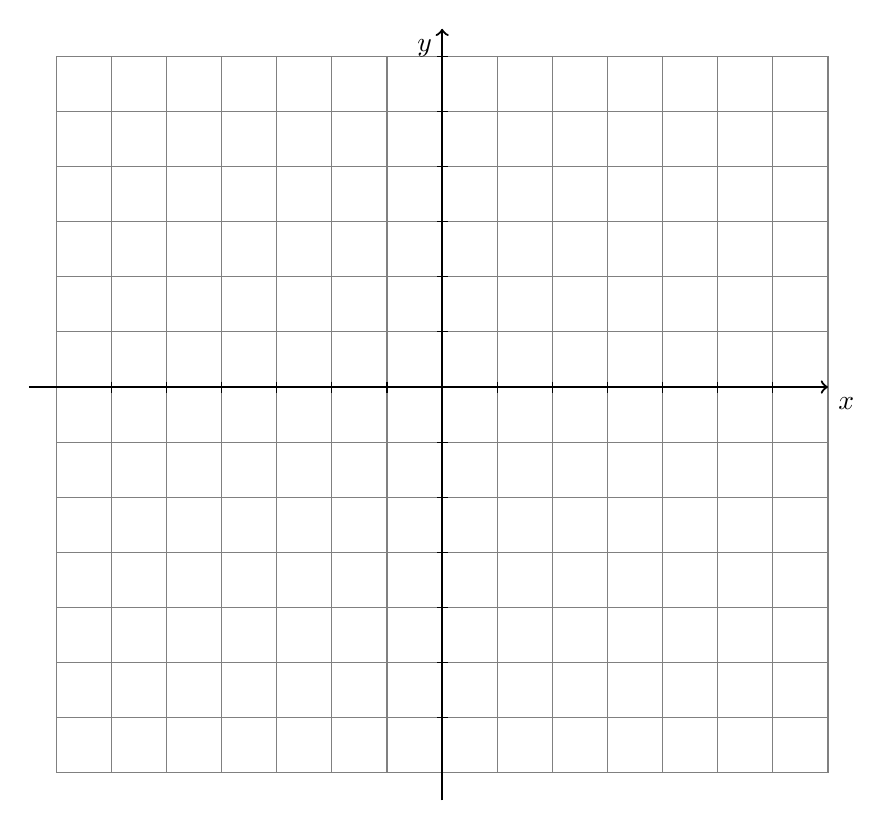
\begin{tikzpicture}[y=.7cm, x=0.7cm,font=\sffamily]
    %% ticks
    \draw[step = 1, gray] (-7,-7) grid (7,6);
    %% axis
    \draw[thick,->] (-7.5,0) -- coordinate (x axis mid) (7,0) node[anchor = north west] {$x$};
    \draw[thick,->] (0,-7.5) -- coordinate (y axis mid) (0,6.5) node[anchor = north east] {$y$};
    \foreach \y in {-6,-5,...,-1,1,2,...,6} {
      \draw (2pt, \y) -- (-2pt, \y);
    }
    \foreach \x in {-6,-5,...,-1,1,2,...,6} {
      \draw (\x,2pt) -- (\x,-2pt);
    }

\end{tikzpicture}



\item Use part $(a)$ to graph the function
  $\displaystyle g(x)=\ln(x)$. Also, graph and label its asymptote.

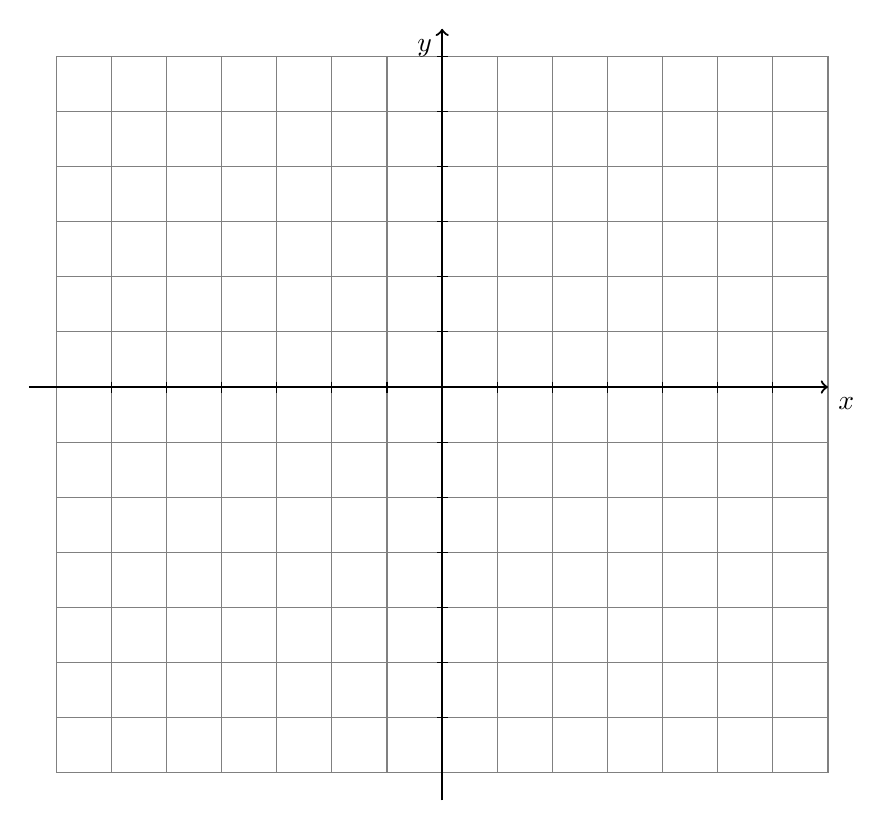
\begin{tikzpicture}[y=.7cm, x=0.7cm,font=\sffamily]
    %% ticks
    \draw[step = 1, gray] (-7,-7) grid (7,6);
    %% axis
    \draw[thick,->] (-7.5,0) -- coordinate (x axis mid) (7,0) node[anchor = north west] {$x$};
    \draw[thick,->] (0,-7.5) -- coordinate (y axis mid) (0,6.5) node[anchor = north east] {$y$};
    \foreach \y in {-6,-5,...,-1,1,2,...,6} {
      \draw (2pt, \y) -- (-2pt, \y);
    }
    \foreach \x in {-6,-5,...,-1,1,2,...,6} {
      \draw (\x,2pt) -- (\x,-2pt);
    }

\end{tikzpicture}


\vfill


\end{enumerate}






\end{enumerate}



